\chapter{Pr�fungen}
\label{pruefungen}
\begin{figure}
	\centering
	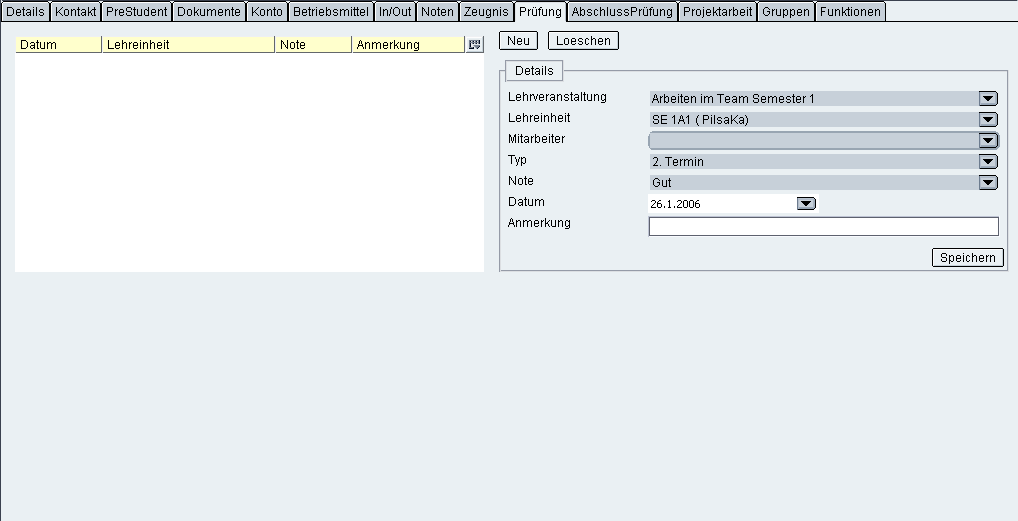
\includegraphics[width=0.75\textwidth]{FAS_Pruefung1.png}
	\caption{Die Karteikarte Pr�fung}
	\label{pruefung1}
\end{figure}
Die Karteikarte \textit{Pr�fung} (siehe Abbildung \ref{pruefung1} besteht aus einem Listenfeld auf der linken Seite und dem Detaildatenbereich auf der rechten Seite und wird f�r die Eintragung von (Wiederholungs-)Pr�fungen verwendet.\\

Wenn eine Pr�fung angelegt wird, wird automatisch die Zeugnisnote aktualisiert.\\
\textbf{Ausnahme:} Wenn das Pr�fungsdatum \underline{vor} dem Benotungsdatum der Zeugnisnote liegt. Hier wird die Pr�fung eingetragen die Zeugnisnote aber nicht ver�ndert. Zus�tzlich erscheint auch eine Warnmeldung, dass die Note nicht ins Zeugnis �bernommen wurde.

\section{Eingabe von Pr�fungen}
Ein Klick auf den Button \textit{Neu} startet den Eingabevorgang. Danach werden die Felder des \textit{Details}-Bereich bef�llt:
\begin{itemize}
	\item Lehrveranstaltung: Die Lehrveranstaltung, in der die Pr�fung erfolgt ist.
	\item Lehreinheit: Hier wird die Lehreinheit ausgew�hlt, die der Student besucht hat.
	\item Mitarbeiter: Der Mitarbeiter, der die Note vergibt.
	\item Typ: Es gibt 3 Pr�fungstypen: den 1.Termin, den 2.Termin (Wiederholung) und die kommissionelle Pr�fung.
	\item Note: Hier kann die Pr�fungsnote ausgew�hlt werden.
	\item Datum: Das Datum der Pr�fung.
	\item Anmerkung: Hier k�nnen zus�tzliche Informationen eingegeben werden.
\end{itemize}
Ein Klick auf den Button \textit{Speichern} beendet mit dem Eintrag der Daten in die Datenbank die Eingabe.

\idee{\textbf{Tipp} Die Pr�fungsnote des Erstantritts mu� im Regelfall nicht eingegeben werden. Bei der Eintragung des Zweitantritts wird der Erstantritt automatisch mit angelegt!}\\
